\documentclass{article}
\usepackage{booktabs}
\usepackage{multirow}
\usepackage{multicol}
\usepackage[table]{xcolor}
\usepackage{colortbl}
\usepackage[backend=biber,natbib=true,style=alphabetic,maxbibnames=50]{biblatex}
\addbibresource{/home/nqbh/reference/bib.bib}
\usepackage[utf8]{vietnam}
\usepackage{tocloft}
\usepackage{tcolorbox}

\setlength{\parindent}{0pt}


\usepackage{minted}

\usepackage{listings}
\usepackage{xcolor}

\lstset{
    language=C++,                    % Ngôn ngữ lập trình
    basicstyle=\ttfamily\footnotesize, % Cỡ chữ nhỏ hơn
    keywordstyle=\color{blue},        % Màu từ khóa
    commentstyle=\color{gray},        % Màu chú thích
    stringstyle=\color{red},          % Màu chuỗi ký tự
    numbers=left,                     % Hiển thị số dòng bên trái
    numberstyle=\tiny\color{gray},    % Định dạng số dòng
    stepnumber=1,                     % Mỗi dòng đều có số dòng
    breaklines=true,                   % Tự động xuống dòng nếu quá dài
    frame=single                      % Đóng khung mã nguồn
}

\renewcommand{\cftsecleader}{\cftdotfill{\cftdotsep}}
\usepackage[colorlinks=true,linkcolor=blue,urlcolor=red,citecolor=magenta]{hyperref}
\usepackage{amsmath,amssymb,amsthm,enumitem,float,graphicx,mathtools,tikz}
\usetikzlibrary{angles,calc,intersections,matrix,patterns,quotes,shadings}
\allowdisplaybreaks
\newtheorem{assumption}{Assumption}
\newtheorem{baitoan}{}
\newtheorem{cauhoi}{Câu hỏi}
\newtheorem{conjecture}{Conjecture}
\newtheorem{corollary}{Corollary}
\newtheorem{dangtoan}{Dạng toán}
\newtheorem{definition}{Definition}
\newtheorem{dinhly}{Định lý}
\newtheorem{dinhnghia}{Định nghĩa}
\newtheorem{example}{Example}
\newtheorem{ghichu}{Ghi chú}
\newtheorem{hequa}{Hệ quả}
\newtheorem{hypothesis}{Hypothesis}
\newtheorem{lemma}{Lemma}
\newtheorem{luuy}{Lưu ý}
\newtheorem{nhanxet}{Nhận xét}
\newtheorem{notation}{Notation}
\newtheorem{note}{Note}
\newtheorem{principle}{Principle}
\newtheorem{problem}{Problem}
\newtheorem{proposition}{Proposition}
\newtheorem{question}{Question}
\newtheorem{remark}{Remark}
\newtheorem{theorem}{Theorem}
\newtheorem{vidu}{Ví dụ}
\usepackage[left=1cm,right=1cm,top=5mm,bottom=5mm,footskip=4mm]{geometry}
\def\labelitemii{$\circ$}
\DeclareRobustCommand{\divby}{%
	\mathrel{\vbox{\baselineskip.65ex\lineskiplimit0pt\hbox{.}\hbox{.}\hbox{.}}}%
}
\setlist[itemize]{leftmargin=*}
\setlist[enumerate]{leftmargin=*}

\title{CHUYÊN ĐỀ: LÝ THUYẾT ĐỒ THỊ} 
\author{Đặng Phúc An Khang\footnote{ E-mail: {\tt ankhangluonvuituoi@gmail.com}. Tây Ninh, Việt Nam.}}
\date{\today}

\begin{document}
\maketitle
\begin{abstract}
	
	
	\textbf{Code:}
	\begin{quote}
		\begin{itemize}
			\item C{\tt/}C++: \url{https://github.com/GrootTheDeveloper/OLP-ICPC/tree/master/2025/C%2B%2B}.
			\item Python: \url{}\\
		\end{itemize}
	\end{quote}
	
	\textbf{Tài khoản trên các Online Judge:}
	\begin{quote}
    	\begin{itemize}
			\item Codeforces: \url{https://codeforces.com/profile/vuivethoima}.
			\item VNOI: \url{oj.vnoi.info/user/Groot}.
			\item IUHCoder: \url{oj.iuhcoder.com/user/ankhang2111}.
			\item MarisaOJ: \url{https://marisaoj.com/user/grootsiuvip/submissions}.
			\item CSES: \url{https://cses.fi/user/212174}.
			\item UMTOJ: \url{sot.umtoj.edu.vn/user/grootsiuvip}.
			\item SPOJ: \url{www.spoj.com/users/grootsiuvip/}.
			\item POJ: \url{http://poj.org/userstatus?user_id=vuivethoima}.
			\item ATCoder: \url{https://atcoder.jp/users/grootsiuvip}
			\item OnlineJudge.org: \url{vuivethoima}
			\item updating...
		\end{itemize}
	\end{quote}
    
\end{abstract}
\tableofcontents

%------------------------------------------------------------------------------%

\section{Preliminaries -- Kiến thức chuẩn bị}

\textbf{\textsf{Resources -- Tài nguyên.}}
\begin{enumerate}
	\item \cite{CP10}. \textit{CP10. Competitive Programming} \url{https://drive.google.com/drive/folders/1MTEVHT-7nBnMJ7C9LgyAR_pEVSE3FlKz?fbclid=IwAR3TovIj2rKCRe1a4oZxW-LQCoEoVkipVAvCzwrr0nJ6GzcAd47P6LO1Rwc}
	
	\item \cite{cp-algorithms}. \textit{Algorithms for Competitive Programming} \url{https://cp-algorithms.com}

    \item \cite{VNOI-WIKI}. \textit{Thư viện VNOI} \url{https://wiki.vnoi.info}



\end{enumerate}


%------------------------------------------------------------------------------%
\section{Kiến thức}
\subsection{Giới thiệu về đồ thị và thuật toán DFS}

\subsubsection{Lý thuyết đồ thị là gì?}

Lý thuyết đồ thị là một nhánh của toán học, cụ thể thuộc toán rời rạc. Lý thuyết đồ thị chuyên nghiên cứu các bài toán liên quan đến việc biểu diễn và phân tích các sự vật, hiện tượng hoặc trạng thái có mối quan hệ lẫn nhau thông qua mô hình đồ thị.\\

\textbf{Một số minh họa điển hình:} Mạng lưới giao thông, cây phả hệ (cây gia phả), mạng máy tính, sơ đồ tổ chức, v.v.

\subsubsection{Một số khái niệm căn bản trong lý thuyết đồ thị}

\begin{enumerate}
    \item \textbf{Đỉnh:} Được biểu diễn nhằm mục đích thể hiện sự vật, sự việc hay một trạng thái.
    \item \textbf{Cạnh:} Biểu diễn cho mối quan hệ giữa 2 đỉnh với nhau. \textbf{Lưu ý:} Giữa 2 đỉnh trong đồ thị có thể có cạnh, không có, hoặc có thể có nhiều cạnh với nhau. Cạnh được chia thành 2 dạng:
    \begin{enumerate}
        \item \textbf{Cạnh vô hướng:} Nếu một cạnh vô hướng nối 2 đỉnh $u$ và $v$, thì $u$ có thể đến $v$ trực tiếp vầ ngược lại.
        \item \textbf{Cạnh có hướng:} Nếu một cạnh có hướng nối từ đỉnh $u$ đến đỉnh $v$, thì ta có thể đi trực tiếp từ $u$ đến $v$, nhưng không thể đi ngược lại từ $v$ đến $u$ trừ khi có một cạnh khác từ $v$ đến $u$.
    \end{enumerate}
    \item \textbf{Đường đi:} Một đường đi là một danh sách các đỉnh $x_1, x_2, x_3, x_4,\dots, x_k$. Trong đó 2 đỉnh $x_i$ và $x_{i + 1}$ thì có một đường nối trực tiếp để đi từ $x_i$ $\rightarrow$ $x_{i + 1}$.
    \item \textbf{Trọng số:} Là một giá trị trên cạnh (hoặc trên đỉnh) nhằm thể hiện một thông số nào đó với bài toán ta đang xét.
\end{enumerate}

\subsubsection{Danh sách kề}

Một trong những cách phổ biến để biểu diễn đồ thị là sử dụng \textbf{danh sách kề (adjacency list)}. Cách biểu diễn này đặc biệt hiệu quả đối với đồ thị thưa \href{https://en.m.wikipedia.org/wiki/Sparse_graph}{(sparse graph)}.


Cụ thể, ta sử dụng cấu trúc dữ liệu \texttt{vector<int> adj[u]} trong C++, trong đó:

\begin{itemize}
    \item Mỗi phần tử \texttt{adj[u]} là một vector chứa các đỉnh kề với đỉnh $u$.
    \item Nghĩa là nếu có cạnh nối từ đỉnh $u$ đến đỉnh $v$ thì $v$ sẽ xuất hiện trong \texttt{adj[u]}.
    \item Đối với đồ thị vô hướng, nếu có cạnh giữa $u$ và $v$ thì cả $v \in \texttt{adj}[u]$ và $u \in \texttt{adj}[v]$.
\end{itemize}

\textbf{Ví dụ:}

Giả sử đồ thị vô hướng có các cạnh: $(1,2)$, $(1,3)$, $(2,4)$ thì danh sách kề sẽ là:

\begin{align*}
\texttt{adj[1]} &= \{2, 3\} \\
\texttt{adj[2]} &= \{1, 4\} \\
\texttt{adj[3]} &= \{1\} \\
\texttt{adj[4]} &= \{2\}
\end{align*}

\begin{figure}[H]
    \centering
    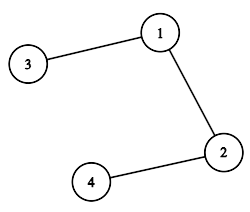
\includegraphics[width=0.2\textwidth]{img/b1/adjlist.png}
    \caption{Minh họa danh sách kề của đồ thị vô hướng vừa mô tả}
    \label{fig:adjlist}
\end{figure}

Cách biểu diễn này có độ phức tạp về bộ nhớ là $\mathcal{O}(n + m)$, với $n$ là số đỉnh và $m$ là số cạnh.

\subsubsection{Chu trình (Cycle)}
Một \textbf{chu trình} là một đường đi bắt đầu và kết thúc tại cùng một đỉnh, trong đó không có đỉnh nào khác (ngoại trừ đỉnh đầu/cuối) được lặp lại.

\begin{itemize}
    \item Trong đồ thị vô hướng: chu trình là dãy đỉnh $v_1 \rightarrow v_2 \rightarrow \dots \rightarrow v_k \rightarrow v_1$ với $k \geq 3$.
    \item Trong đồ thị có hướng: các cung phải có hướng phù hợp với trình tự chu trình.
\end{itemize}

Một chu trình được gọi là \textit{chu trình đơn giản} nếu không có cạnh hoặc đỉnh nào bị lặp lại (trừ đỉnh đầu/cuối).

\begin{figure}[H]
    \centering
    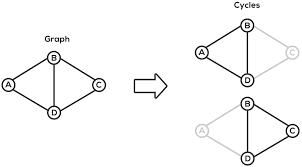
\includegraphics[width=0.4\textwidth]{img/b1/cycle.png}
    \caption{Minh họa chu trình của đồ thị vô hướng}
    \label{fig:cycle}
\end{figure}

\subsubsection{Thành phần liên thông \href{https://www.geeksforgeeks.org/dsa/strongly-connected-components/}{(Connected Component)}}
Một \textbf{thành phần liên thông} là một tập con các đỉnh sao cho giữa mọi cặp đỉnh trong đó đều tồn tại một đường đi.

\begin{itemize}
    \item Với đồ thị vô hướng: liên thông nếu có đường đi giữa mọi cặp đỉnh.
    \item Với đồ thị có hướng:
        \begin{itemize}
            \item \textit{Liên thông mạnh} nếu tồn tại đường đi theo chiều từ mọi đỉnh đến mọi đỉnh khác.
            \item \textit{Liên thông yếu} nếu bỏ hướng trên các cạnh thì đồ thị trở nên liên thông.
        \end{itemize}
\end{itemize}

\begin{figure}[H]
    \centering
    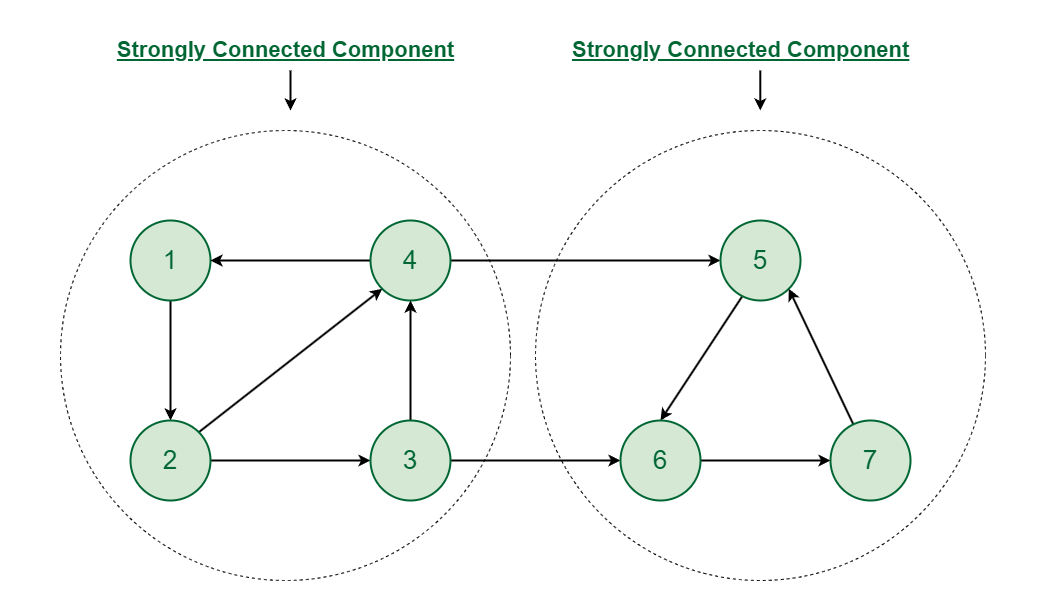
\includegraphics[width=0.4\textwidth]{img/b1/SCC.png}
    \caption{Minh họa thành phần liên thông mạnh của đồ thị có hướng}
    \label{SCC}
\end{figure}

\subsubsection{Bậc của đỉnh (Degree)}
\begin{itemize}
    \item Trong đồ thị vô hướng, bậc của một đỉnh là số cạnh nối với nó.
    \item Trong đồ thị có hướng:
        \begin{itemize}
            \item \textit{Bậc vào} (in-degree): số cung đi vào đỉnh.
            \item \textit{Bậc ra} (out-degree): số cung đi ra từ đỉnh.
        \end{itemize}
\end{itemize}

\subsubsection{Đường đi đơn giản (Simple Path)}
Một \textbf{đường đi đơn giản} là đường đi không đi qua một đỉnh nào hai lần (trừ khi là chu trình).

\subsubsection{Cây (Tree)}
Một \textbf{cây} là một đồ thị vô hướng liên thông và không có chu trình.

Tính chất quan trọng của cây:
\begin{itemize}
    \item Với $n$ đỉnh, cây có đúng $n - 1$ cạnh.
    \item Có duy nhất một đường đi giữa hai đỉnh bất kỳ.
\end{itemize}

\begin{figure}[H]
    \centering
    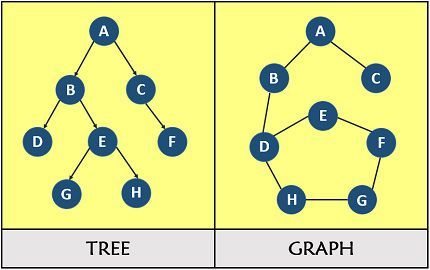
\includegraphics[width=0.4\textwidth]{img/b1/treegraph.png}
    \caption{Phân biệt Cây và Đồ thị (không phải cây)}
    \label{treegraph}
\end{figure}

\subsubsection{Đồ thị vô chu trình (Acyclic Graph).}
Đồ thị gọi là \textbf{vô chu trình} nếu không tồn tại chu trình nào trong nó.
\begin{itemize}
    \item Với đồ thị \textbf{vô hướng}, một đồ thị được xem là \textbf{Acyclic Graph} nếu không tồn tại dãy các đỉnh $v_1 \rightarrow v_2 \rightarrow \dots \rightarrow v_k \rightarrow v_1$ với $k \geq 3$ và các cạnh liên tiếp nối các đỉnh đó.
    \item Một đồ thị vô hướng đơn giản gồm hai đỉnh được nối với nhau bằng một cạnh cũng là một \textbf{Acyclic Graph}, vì không tồn tại chu trình nào (phải có ít nhất 3 đỉnh để hình thành chu trình trong đồ thị vô hướng).
    \item Đồ thị có hướng vô chu trình gọi là \textbf{DAG} (Directed Acyclic Graph). Nghĩa là một đồ thị có hướng không chứa bất kỳ chu trình nào tuân theo chiều các cung.
    \item Cây là một DAG, nhưng không phải tất cả DAG đều là cây.
\end{itemize}

\begin{figure}[H]
    \centering
    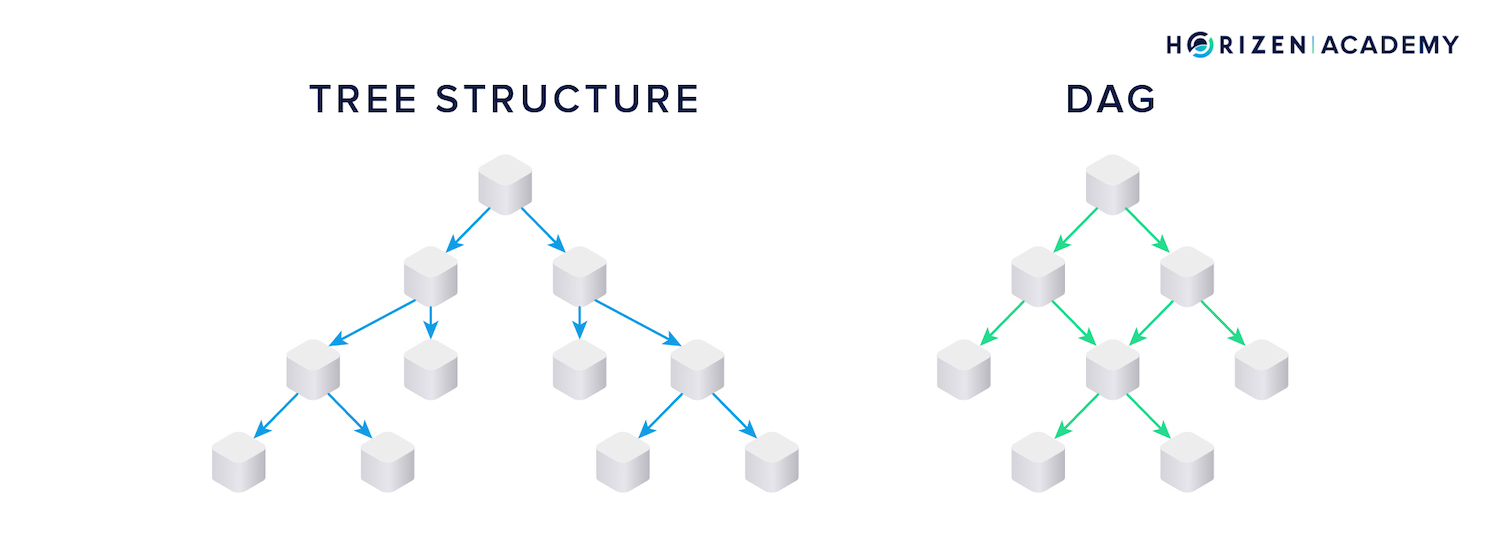
\includegraphics[width=0.6\textwidth]{img/b1/treevsdag.jpg}
    \caption{Phân biệt Cây và DAG}
\end{figure}

\subsubsection{Đồ thị đơn (Simple Graph).}
Đồ thị đơn là đồ thị không có \emph{cạnh lặp} giữa cùng một cặp đỉnh và không có \emph{khuyên} (loop – cạnh nối đỉnh với chính nó).

\subsubsection{Đa đồ thị (Multigraph).}
Đa đồ thị cho phép tồn tại \emph{nhiều cạnh song song} giữa hai đỉnh và/hoặc khuyên.  
Thường dùng để mô hình hoá các mạng có nhiều kênh kết nối.

\begin{figure}[H]
    \centering
    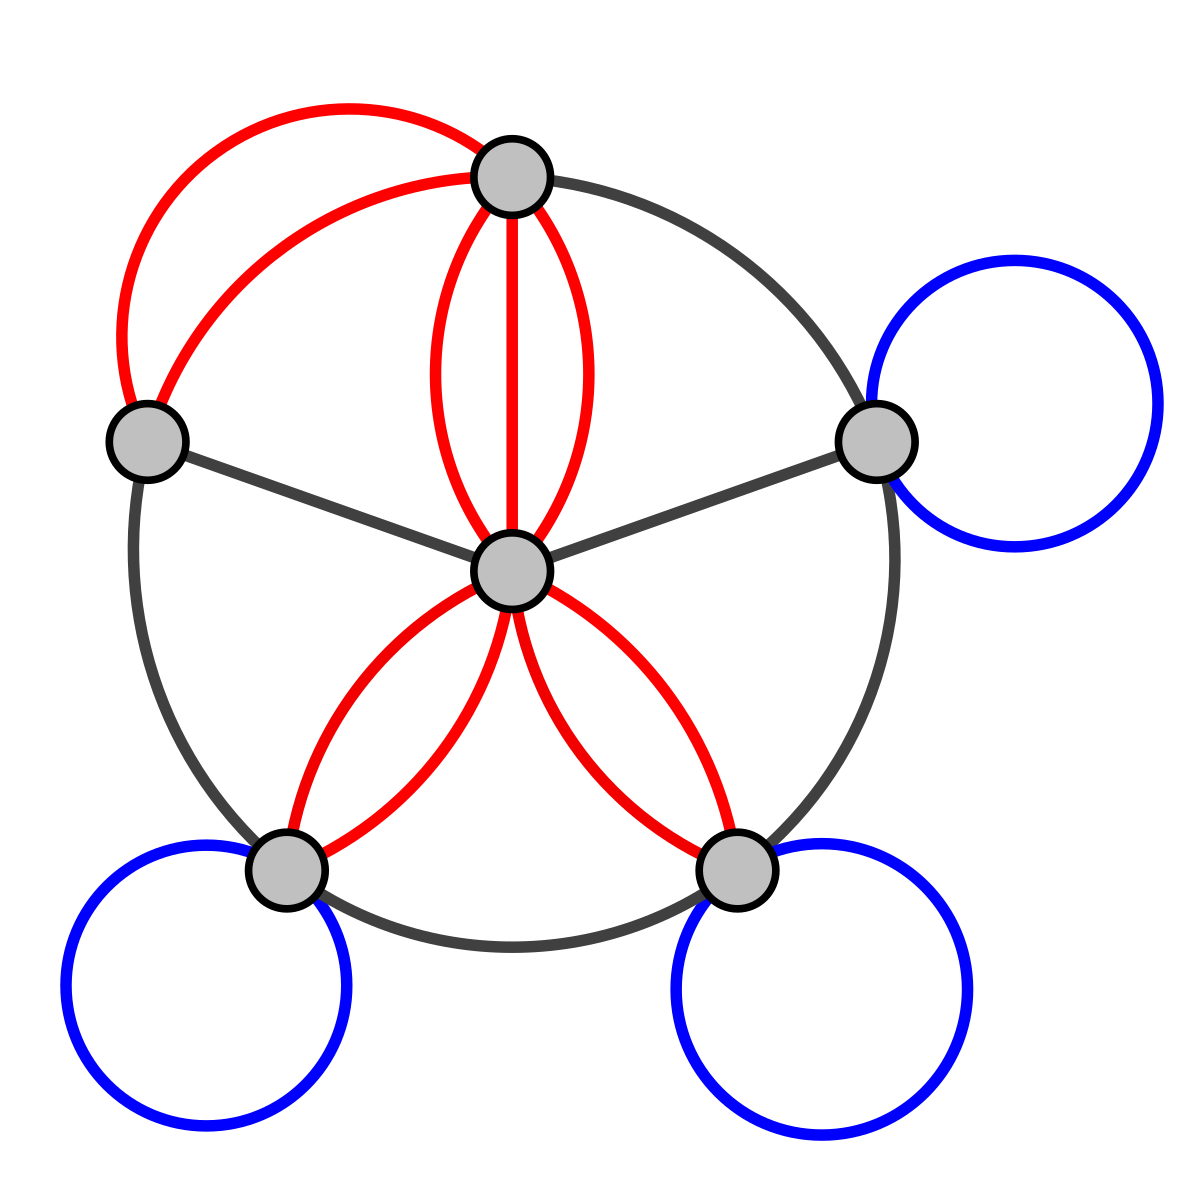
\includegraphics[width=0.2\textwidth]{img/b1/multigraph.png}
    \caption{Minh họa Đa đồ thị}
    \label{multigraph}
\end{figure}

\subsubsection{Đồ thị đầy đủ (Complete Graph).}
Đồ thị vô hướng \(K_n\) có \(n\) đỉnh, trong đó mọi cặp đỉnh phân biệt đều được nối bởi một cạnh. 

Số cạnh là \(\dfrac{n(n-1)}{2}\).  

Đồ thị có hướng đầy đủ có \(n(n-1)\) cung.

\begin{figure}[H]
    \centering
    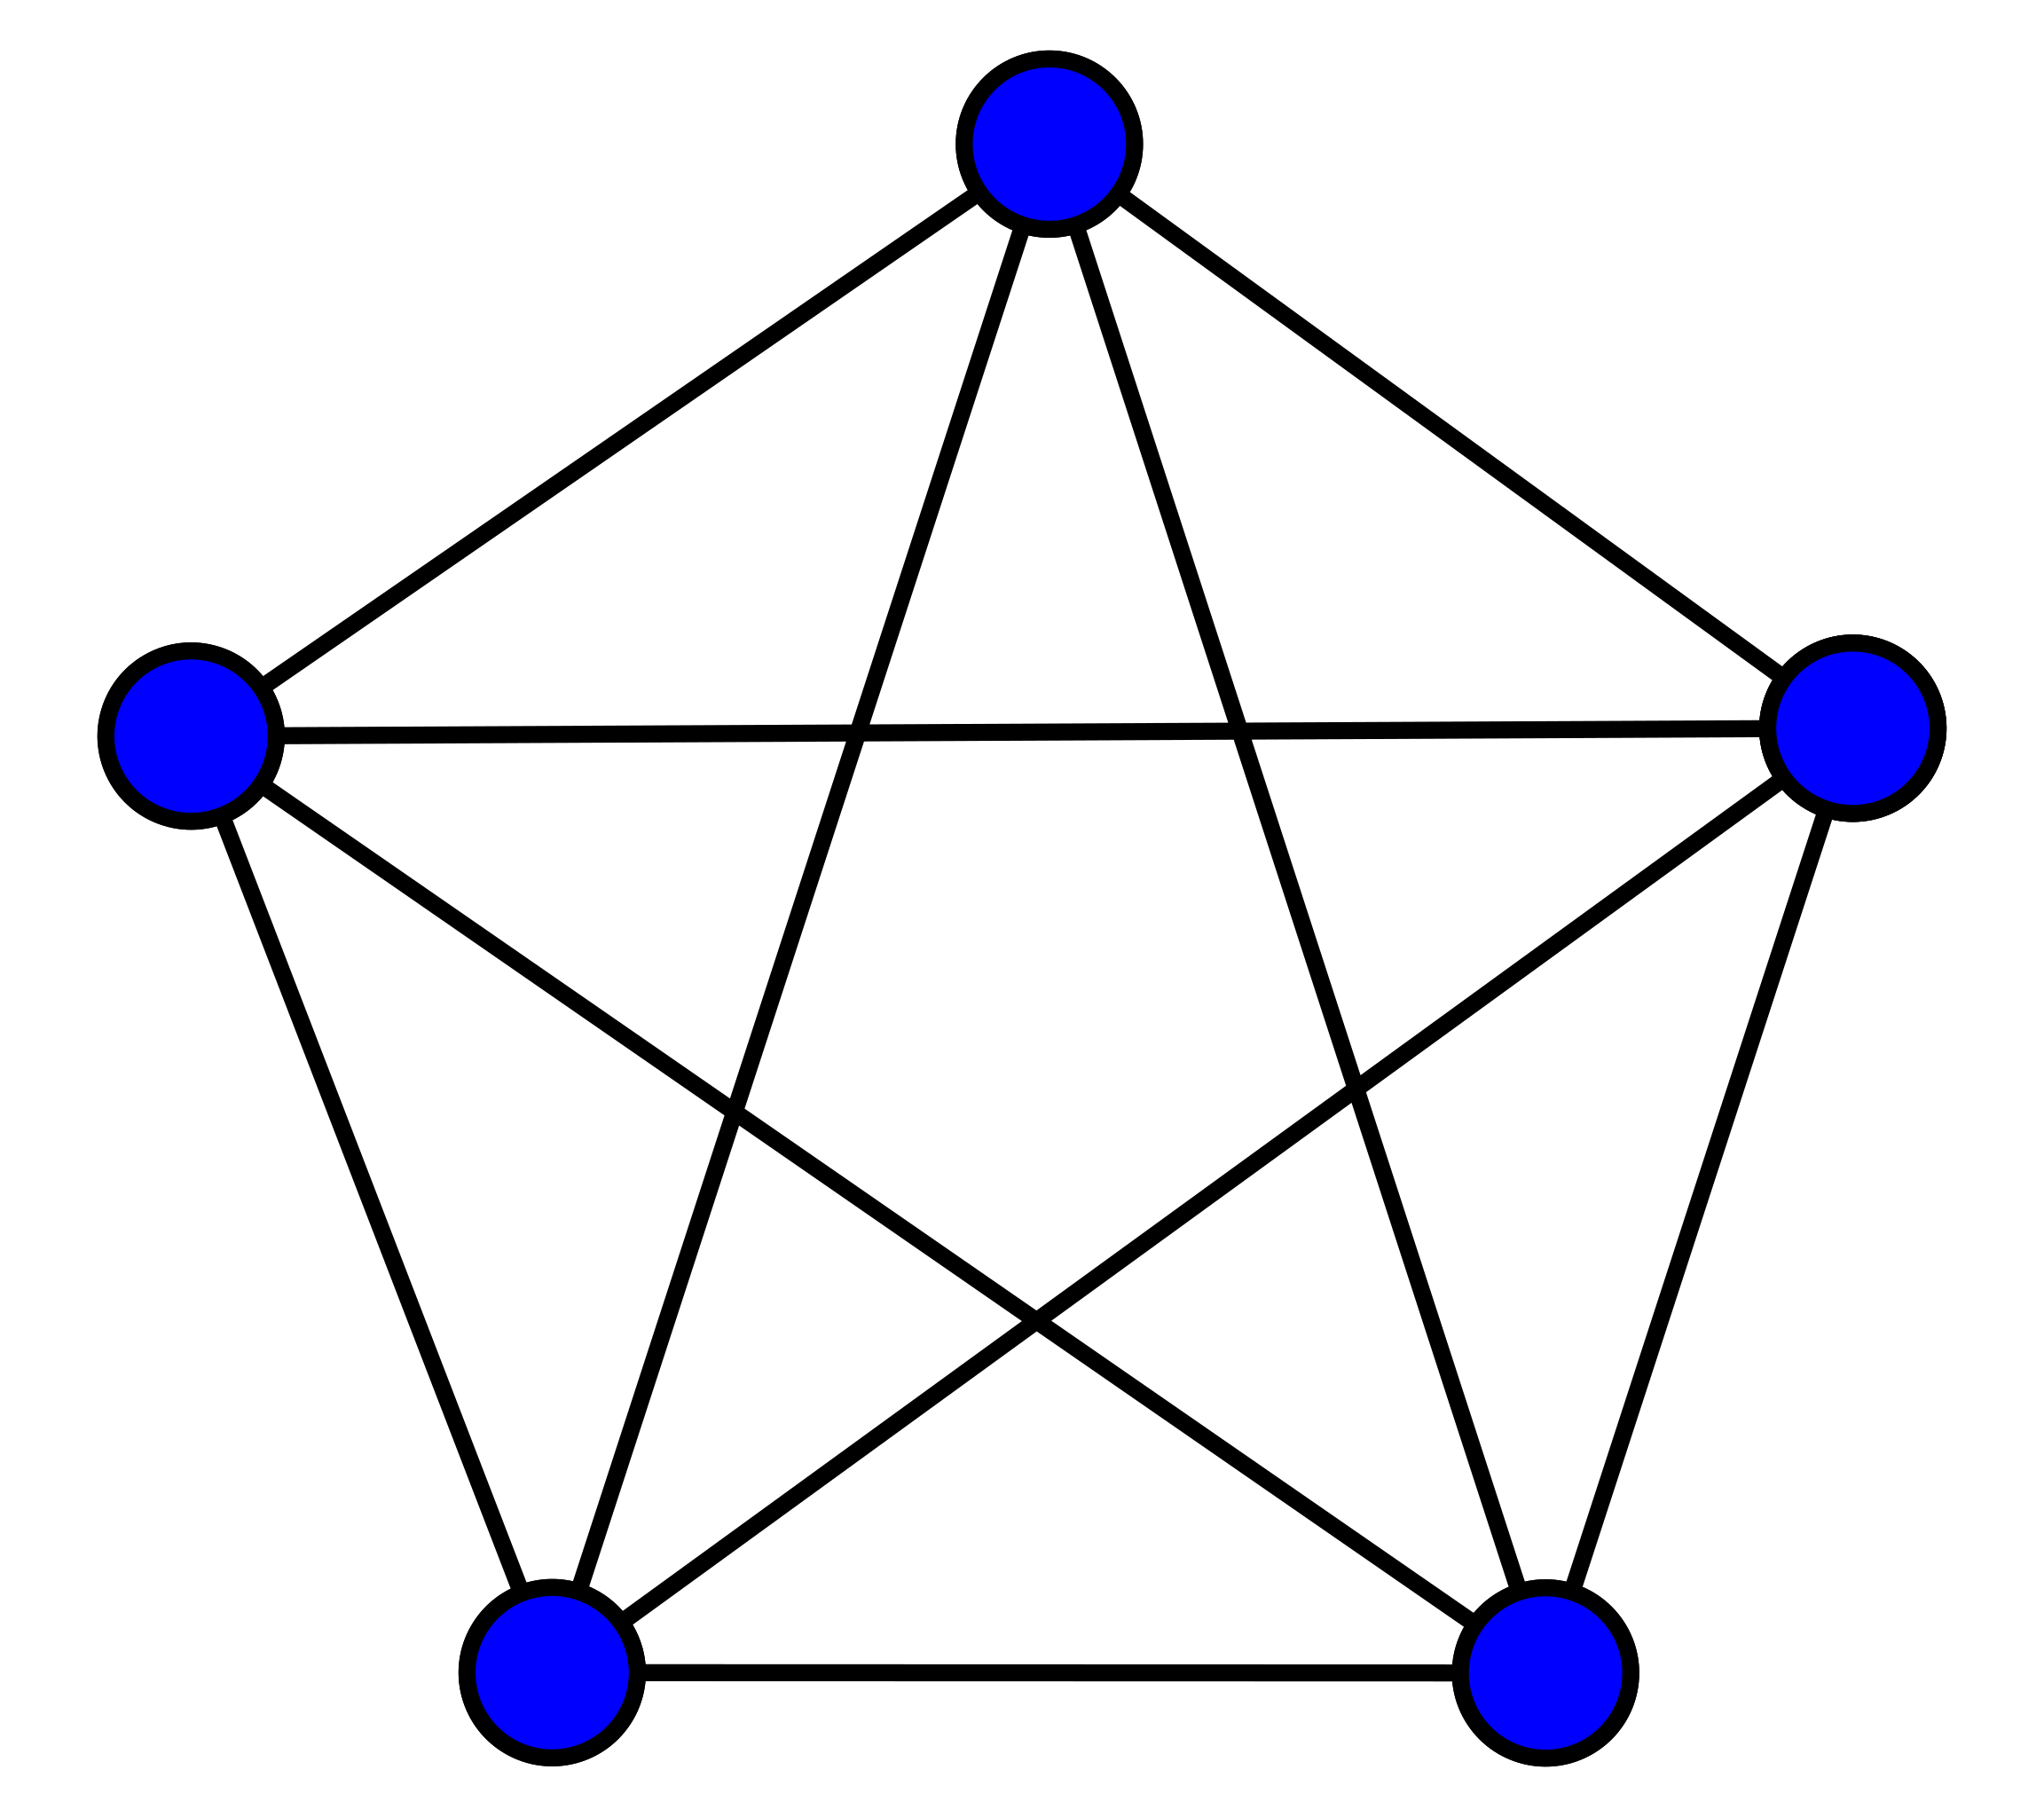
\includegraphics[width=0.2\textwidth]{img/b1/CG.png}
    \caption{Minh họa đồ thị đầy đủ}
    \label{CG}
\end{figure}

\subsubsection{Đồ thị hai phía (Bipartite Graph).}
Một \textbf{đồ thị hai phía} là đồ thị mà tập đỉnh có thể chia thành hai tập rời $U$ và $V$ sao cho mọi cạnh đều nối một đỉnh từ $U$ đến một đỉnh từ $V$.

\begin{figure}[H]
    \centering
    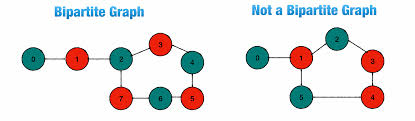
\includegraphics[width=0.5\textwidth]{img/b1/biparitegraph.png}
    \caption{Phân biệt đồ thị hai phía}
    \label{biparite}
\end{figure}

\subsubsection{Đồ thị hai phía đầy đủ (Complete Bipartite Graph).}
Cho hai tập đỉnh rời \(U\) và \(V\) với \(|U| = m,\;|V| = n\).  
Đồ thị \(K_{m,n}\) chứa mọi cạnh nối một đỉnh của \(U\) với một đỉnh của \(V\) và \emph{không có cạnh nội bộ} trong \(U\) hay \(V\).  
Tổng số cạnh: \(m\,n\).

\begin{figure}[H]
    \centering
    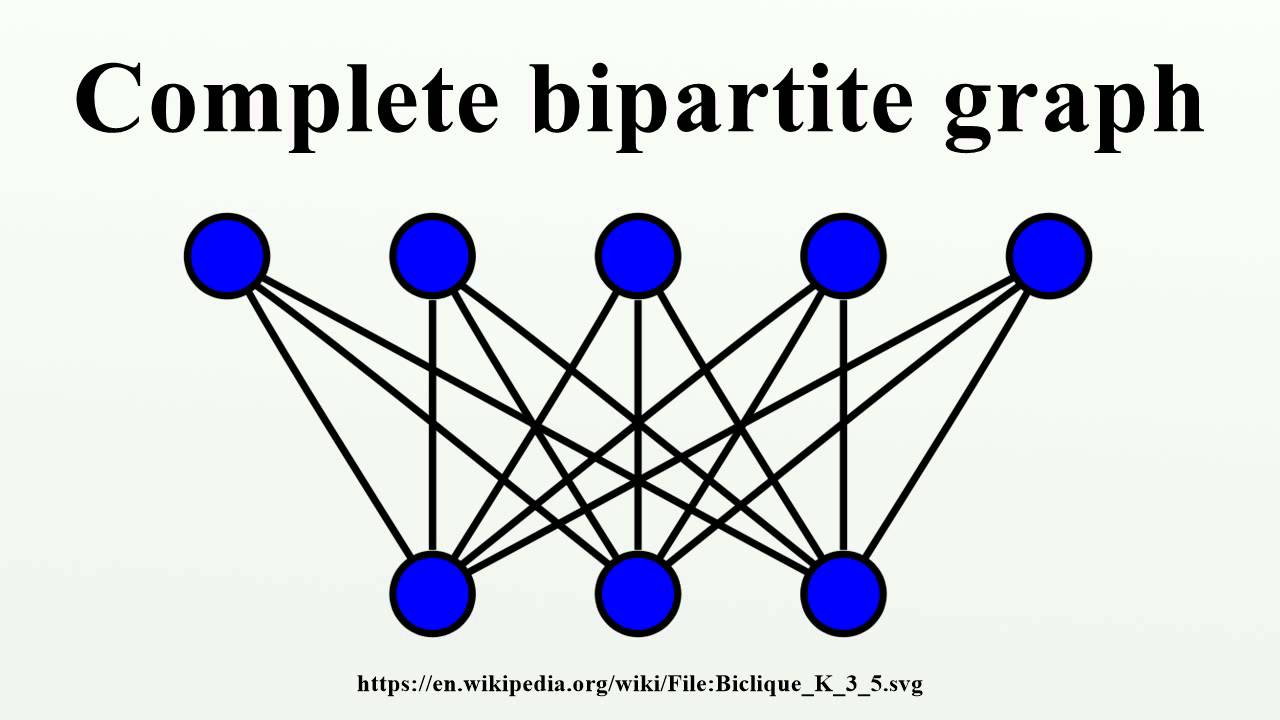
\includegraphics[width=0.4\textwidth]{img/b1/completebiparitegraph.png}
    \caption{Minh họa đồ thị hai phía đầy đủ}
    \label{CBG}
\end{figure}

\subsubsection{Đồ thị vòng (Cycle Graph)}
Đồ thị vòng ký hiệu \(C_n\;(n \ge 3)\) là đồ thị vô hướng gồm \(n\) đỉnh
\(\{v_1,v_2,\dots ,v_n\}\) và \(n\) cạnh
\[
E = \bigl\{\{v_1,v_2\},\{v_2,v_3\},\dots ,\{v_{n-1},v_n\},\{v_n,v_1\}\bigr\}.
\]

\begin{itemize}
    \item Mỗi đỉnh có bậc \(2\) – \(C_n\) là đồ thị \(2\)-chính quy.
    \item \(C_n\) chứa đúng một chu trình đơn giản độ dài \(n\).
    \item \(C_n\) là \textbf{bipartite} khi và chỉ khi \(n\) chẵn.
    \item Số cạnh \(m = n\); số đỉnh \(n\); đường kính (diameter)  
          \(\operatorname{diam}(C_n) = \bigl\lfloor n/2 \bigr\rfloor\).
    \item Tồn tại cây khung nhỏ nhất với trọng số tổng bằng \(n-1\) nếu mọi cạnh có trọng số \(1\).
\end{itemize}

\begin{figure}[H]
    \centering
    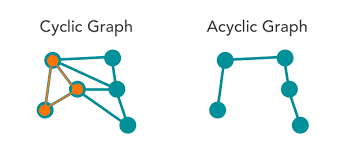
\includegraphics[width=0.4\textwidth]{img/b1/CGvsAG.png}
    \caption{Minh họa CG và AG}

\end{figure}
\subsubsection{Rừng (Forest).}
Một \textbf{rừng} là đồ thị vô hướng \emph{không chứa chu trình} nhưng \emph{không nhất thiết liên thông}.  
Mỗi thành phần liên thông của rừng là một \textbf{cây}.  
Nếu rừng có \(c\) cây và \(n\) đỉnh, nó có đúng \(n-c\) cạnh.


\begin{figure}[H]
    \centering
    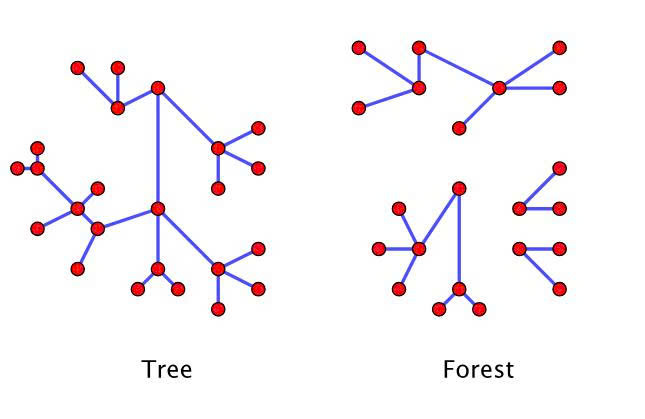
\includegraphics[width=0.4\textwidth]{img/b1/treevsforest.jpg}
    \caption{Tree vs Forest}    
\end{figure}


\subsection{Thuật toán DFS}

Thuật toán DFS (Depth-First Search – Duyệt theo chiều sâu) là một trong những thuật toán cơ bản để duyệt hoặc tìm kiếm trên đồ thị. Ý tưởng chính là xuất phát từ một đỉnh ban đầu, đi sâu theo từng nhánh con của đồ thị cho đến khi không còn đỉnh nào có thể đi tiếp, sau đó quay lui để khám phá các nhánh khác.

DFS có thể được cài đặt đệ quy hoặc sử dụng ngăn xếp. Nó thường được dùng để:

\begin{itemize}
    \item Kiểm tra tính liên thông của đồ thị
    \item Tìm thành phần liên thông
    \item Phát hiện chu trình
    \item Tìm đường đi trong mê cung hoặc đồ thị
\end{itemize}

\subsubsection{Ý tưởng cài đặt thuật toán DFS}

DFS thường được cài đặt bằng đệ quy hoặc sử dụng ngăn xếp. Trong cài đặt đệ quy, ta cần một mảng đánh dấu để theo dõi các đỉnh đã được thăm nhằm tránh lặp vô hạn trong trường hợp đồ thị có chu trình.

\textbf{Các bước cơ bản trong cài đặt DFS đệ quy:}

\begin{enumerate}
    \item Khởi tạo một mảng \texttt{visited[]} để đánh dấu các đỉnh đã được duyệt, với ý nghĩa: \texttt{visited[u] = true / false} nếu đỉnh $u$ đã thăm / chưa thăm.
    \item Gọi hàm \texttt{DFS(u)} tại đỉnh bắt đầu $u$.
    \item Trong mỗi lần gọi:
    \begin{itemize}
        \item Đánh dấu \texttt{visited[u] = true}.
        \item Duyệt qua tất cả các đỉnh kề $v$ của $u$:
        \begin{itemize}
            \item Nếu $v$ chưa được thăm (\texttt{visited[v] == false}), đệ quy gọi \texttt{DFS(v)}.
        \end{itemize}
    \end{itemize}
\end{enumerate}

\subsubsection{Cài đặt DFS sử dụng đệ quy trong C++}

\begin{lstlisting}[language=C++, caption={Thuật toán DFS sử dụng đệ quy}, label={code:dfs}]
#include <iostream>
#include <vector>
using namespace std;

const int MAXN = 100005; // So dinh toi da
vector<int> adj[MAXN];   // Danh sach ke
bool visited[MAXN];      // Mang danh dau

void DFS(int u) {
    visited[u] = true;
    cout << "Tham dinh: " << u << endl;
    for (int v : adj[u]) {
        if (!visited[v]) {
            DFS(v);
        }
    }
}
int main() {
    int n, m; // so dinh va so canh
    cin >> n >> m;
    for (int i = 0; i < m; i++) {
        int u, v;
        cin >> u >> v;
        adj[u].push_back(v);
        adj[v].push_back(u); // Neu la do thi vo huong
    }
    for (int i = 1; i <= n; i++) {
        visited[i] = false;
    }
    // Goi DFS tu dinh 1 (hoac 1 dinh bat ky)
    DFS(1);

    return 0;
}
\end{lstlisting}

\textbf{Độ phức tạp: } $\mathcal{O}(V + E)$ với $V$ là số đỉnh, $E$ là số cạnh.

\subsubsection{Bài tập}
\paragraph{2.2.4.1. \href{https://www.spoj.com/problems/MAKEMAZE/}{MAKEMAZE}}

\textbf{Đề bài}

Một mê cung hợp lệ là một mê cung có chính xác 1 lối vào và 1 lối ra  và phải tồn tại ít nhất một đường đi thỏa mãn từ lối vào đến lối ra. Cho một mê cung, hãy chỉ ra rằng mê cung có hợp lệ hay không. Nếu có, in ``valid'', ngược lại in ``invalid''

\textbf{Input}

Dòng đầu chứa một số nguyên $t$ $(1 \leq t \leq 10^4)$ là số lượng test cases. Sau đó với mỗi test case, dòng đầu chứa 2 số nguyên $m$ $(1 \leq m \leq 20)$ và $n$ $(1 \leq n \leq 20)$, lần lượt là số lượng hàng và cột trong mê cung. Sau đó, là mê cung $M$ với kích thước $m$ x $n$. $M[i][j] = '\#'$ đại diện cho bức tường, $M[i][j] = '.'$ đại diện cho ô trống có thể đi vào được.

\textbf{Output}

Với mỗi test case, tìm xem mê cung tương ứng là ``invalid'' hay ``valid''

\textbf{Example}

1\\
4 4 \\
\#\#\#\# \\
\#...  \\
\#.\#\# \\
\#.\#\# \\

$\rightarrow$ ``valid''

\textbf{Phân tích bài toán}

Vì mê cung chỉ có chính xác 1 lối vào và 1 lối ra. Trước hết ta cần kiểm tra biên ngoài của mê cung, nếu có chính xác 2 ô '.' thì có thể đó là một mê cung hợp lệ. Ngược lại (có ít hơn hoặc nhiều hơn 1 ô '.' ở biên) ta có thể khẳng định rằng đó không phải là một mê cung hợp lệ. \\

Khi ta đã có giả thuyết rằng mê cung là hợp lệ, ta cần 2 biến \textit{start} và \textit{target} lần lượt lưu lại tọa độ $(x, y)$ của 2 ô ngoài biên. Áp dụng thuật toán DFS tại ô $start$, sau khi DFS nếu \textit{visited[target.first][target.second] = true} thì khẳng định rằng mê chung hợp lệ. Ngược lại, mê cung khônxg hợp lệ.
\begin{lstlisting}[language=C++, caption={Cài đặt C++ bài MAKEMAZE}, label={code:makemaze}]
#include <bits/stdc++.h>
#define int long long
#define endl "\n"
using namespace std;

const int MAXN = 21;
bool visited[MAXN][MAXN];

int dx[4] = {1, -1, 0, 0};
int dy[4] = {0, 0, 1, -1};

void dfs(pair<int, int> start, const vector<vector<char>> &a, int m, int n) {
    auto [x, y] = start;
    visited[x][y] = true;
    for (int i = 0; i < 4; i++) {
        int new_x = dx[i] + x;
        int new_y = dy[i] + y;
        if (new_x >= 1 && new_x <= m && new_y >= 1 && new_y <= n &&
            !visited[new_x][new_y] && a[new_x][new_y] == '.') {
            dfs({new_x, new_y}, a, m, n);
        }
    }
}

signed main() {
    int t; cin >> t;
    while (t--) {
        int m, n; cin >> m >> n;
        vector<vector<char>> a(m + 1, vector<char>(n + 1));
        for (int i = 1; i <= m; i++) {
            for (int j = 1; j <= n; j++) {
                cin >> a[i][j];
                visited[i][j] = false;
            }
        }

        pair<int, int> start = {-1, -1}, target = {-1, -1};
        int cnt = 0;

        for (int i = 1; i <= m; i++) {
            for (int j = 1; j <= n; j++) {
                if ((i == 1 || i == m || j == 1 || j == n) && a[i][j] == '.') {
                    if (start == make_pair(-1LL, -1LL)) start = {i, j};
                    else target = {i, j};
                    cnt++;
                }
            }
        }

        if (cnt != 2) {
            cout << "invalid" << endl;
            continue;
        } else {
            dfs(start, a, m, n);
            if (!visited[target.first][target.second]) cout << "invalid";
            else cout << "valid";
            cout << endl;
        }
    }
    return 0;
}

\end{lstlisting}

\subsection{Topological Sorting}


\subsection{Khớp và Cầu (Joints and Brides)}

\subsection{Thành phần liên thông mạnh (Strongly Connected Components)}

\subsection{Thuật toán BFS}

\subsection{Thuật toán Dijkstra + Heap}

\subsection{Disjoint Set Union (DSU)}

\subsection{Maximum Flow and Maximum Matching}

\subsection{Minimum Cut}
\subsection{Euler Tour}
\subsection{Lowest Common Ancestor}
\subsection{Heavy Light Decomposition}
\subsection{Centroid Decomposition}
\subsection{2-SAT}



\section{Miscellaneous}

\subsection{Contributors}


%------------------------------------------------------------------------------%

\printbibliography[heading=bibintoc]
	
\end{document}